\documentclass[final]{beamer}
\def\bx{\boldsymbol{x}}
\def\bth{\boldsymbol{\theta}}
\def\xbar{\bar{x}}
\def\xbar{\bar{x}}
\def\dstar{\delta^{*}}
\def\xis{\xi^{*}}
\def\psis{\psi^{*}}

\definecolor{Set1Red}{HTML}{E41A1C}
\definecolor{Set1Blue}{HTML}{377EBA}
\definecolor{Set1Green}{HTML}{4DAF4A}

\mode<presentation>
{ \usetheme{jared} }
\usepackage{mathptmx}
\usepackage{amsmath,amsthm, amssymb, latexsym}
\boldmath
\usepackage[english]{babel}
\usepackage[latin1]{inputenc}
\usepackage[orientation=portrait,size=a0,scale=1.4]{beamerposter}
\usepackage{subfigure}
\usepackage{tikz}
\usepackage{sidecap}
\fboxsep1pt

%%%%%%%%%%%%%%%%%%%%%%%%%%%%%%%%%%%%%%%%
\title{BIGGIE: A Distributed Pipeline for Genomic Variant Calling}
\author{Richard Xia$^1$, Sara Sheehan$^1$, Yuchen Zhang$^1$, Ameet Talwalkar$^1$, Matei Zaharia$^1$ 
Jonathan Terhorst$^2$, \\ Michael Jordan$^{1,2}$, Yun S. Song$^{1,2}$, Armando Fox$^1$, David Patterson$^1$}
\institute{$^1$ Computer Science Division, UC Berkeley; $^2$ Department of Statistics, UC Berkeley}
%%%%%%%%%%%%%%%%%%%%%%%%%%%%%%%%%%%%%%%%

\begin{document}

\begin{frame}{}

\begin{columns}
\begin{column}{.98\linewidth}
\begin{block}{Motivation: faster, open-source genome variant calling tools}
	\begin{columns}
       	\begin{column}{.40\linewidth}
		\textbf{\color{berkblue}{Impact:}} \\
		Human genome variation is being used more and more to impact disease diagnosis and treatment, however:
		\begin{itemize}
			\item current tools frequently disagree on variant calls
			\item different types of variation require specialized tools
		\end{itemize}
		\textbf{\color{berkblue}{Current Tools:}}
			\begin{itemize}
				\item GATK [2]: slow and difficult to use
				\item CASAVA [1]: fast, but not free
				\item samtools mpileup [3]: slow and some accuracy issues
			\end{itemize}
		\textbf{\color{berkblue}{Our Goal:}}
			\begin{itemize}
				\item fast, distributed variant caller
				\item separate the genome into regions of high and low complexity and use the right tool for the right region
			\end{itemize}
	\end{column}
	\begin{column}{.58\linewidth}
		\begin{figure}[h!]
  			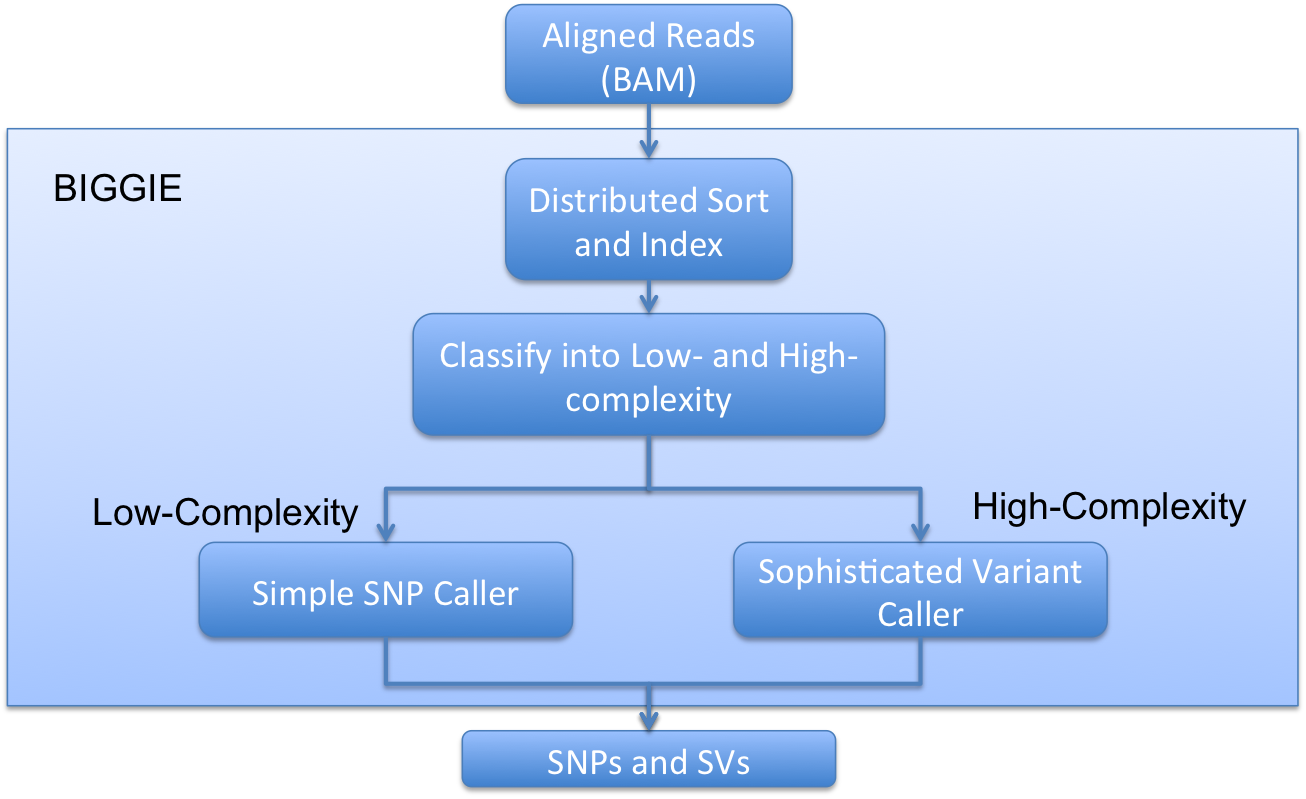
\includegraphics[width=300mm]{figs/pipeline.png}
			\caption{BIGGIE pipeline}
  		\end{figure}
	\end{column}
	\end{columns}
\end{block}
\end{column}
\end{columns}

\vskip.75cm

\begin{columns}[t]
\begin{column}{.48\linewidth}

\begin{block}{Per-base SNP caller}
	\textbf{\color{berkblue}{Main idea:}}
		\begin{itemize}
			\item Distrubted pipeline for variant calling using Spark [4]
			\item Assign a {\em complexity} score to each base
			\item Use a simple SNP caller at bases with a low complexity score 
			\item Use more robust structural variant callers at high complexity bases
		\end{itemize}
	\vspace{3mm}
	\textbf{\color{berkblue}{Complexity region examples:}}
	\begin{figure}
		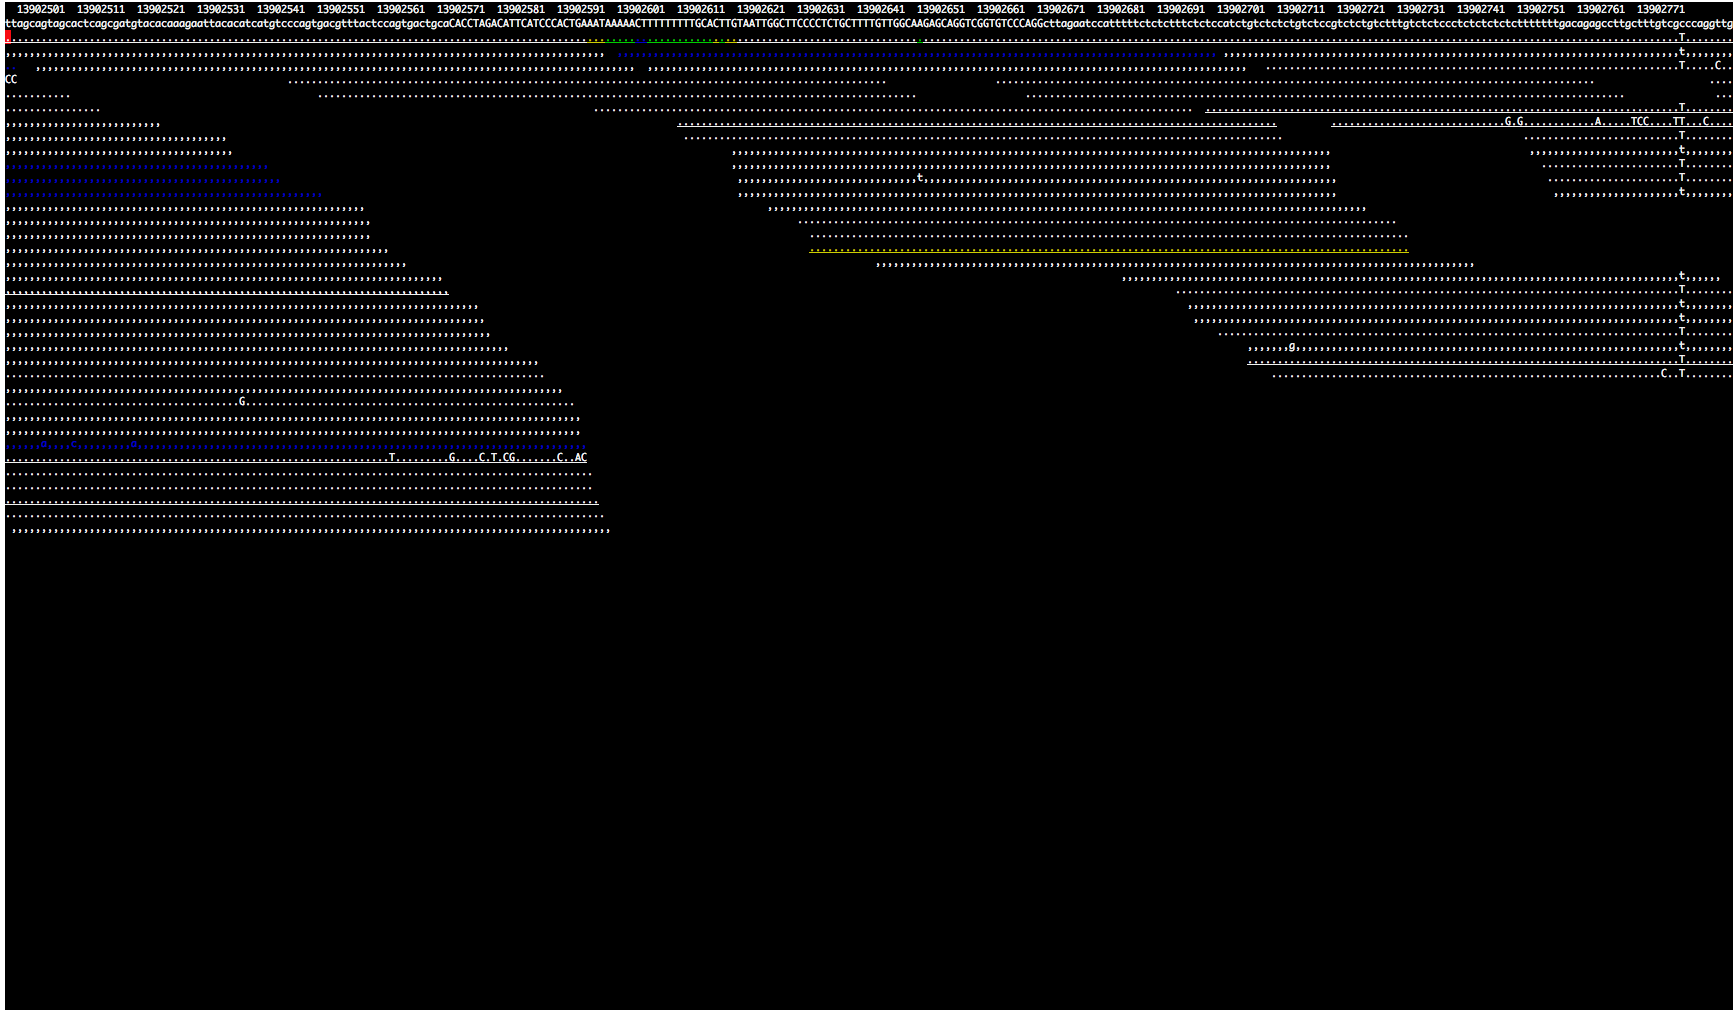
\includegraphics[height=85mm]{figs/tview_low_complexity2_SNP.png} \hspace{10mm}
		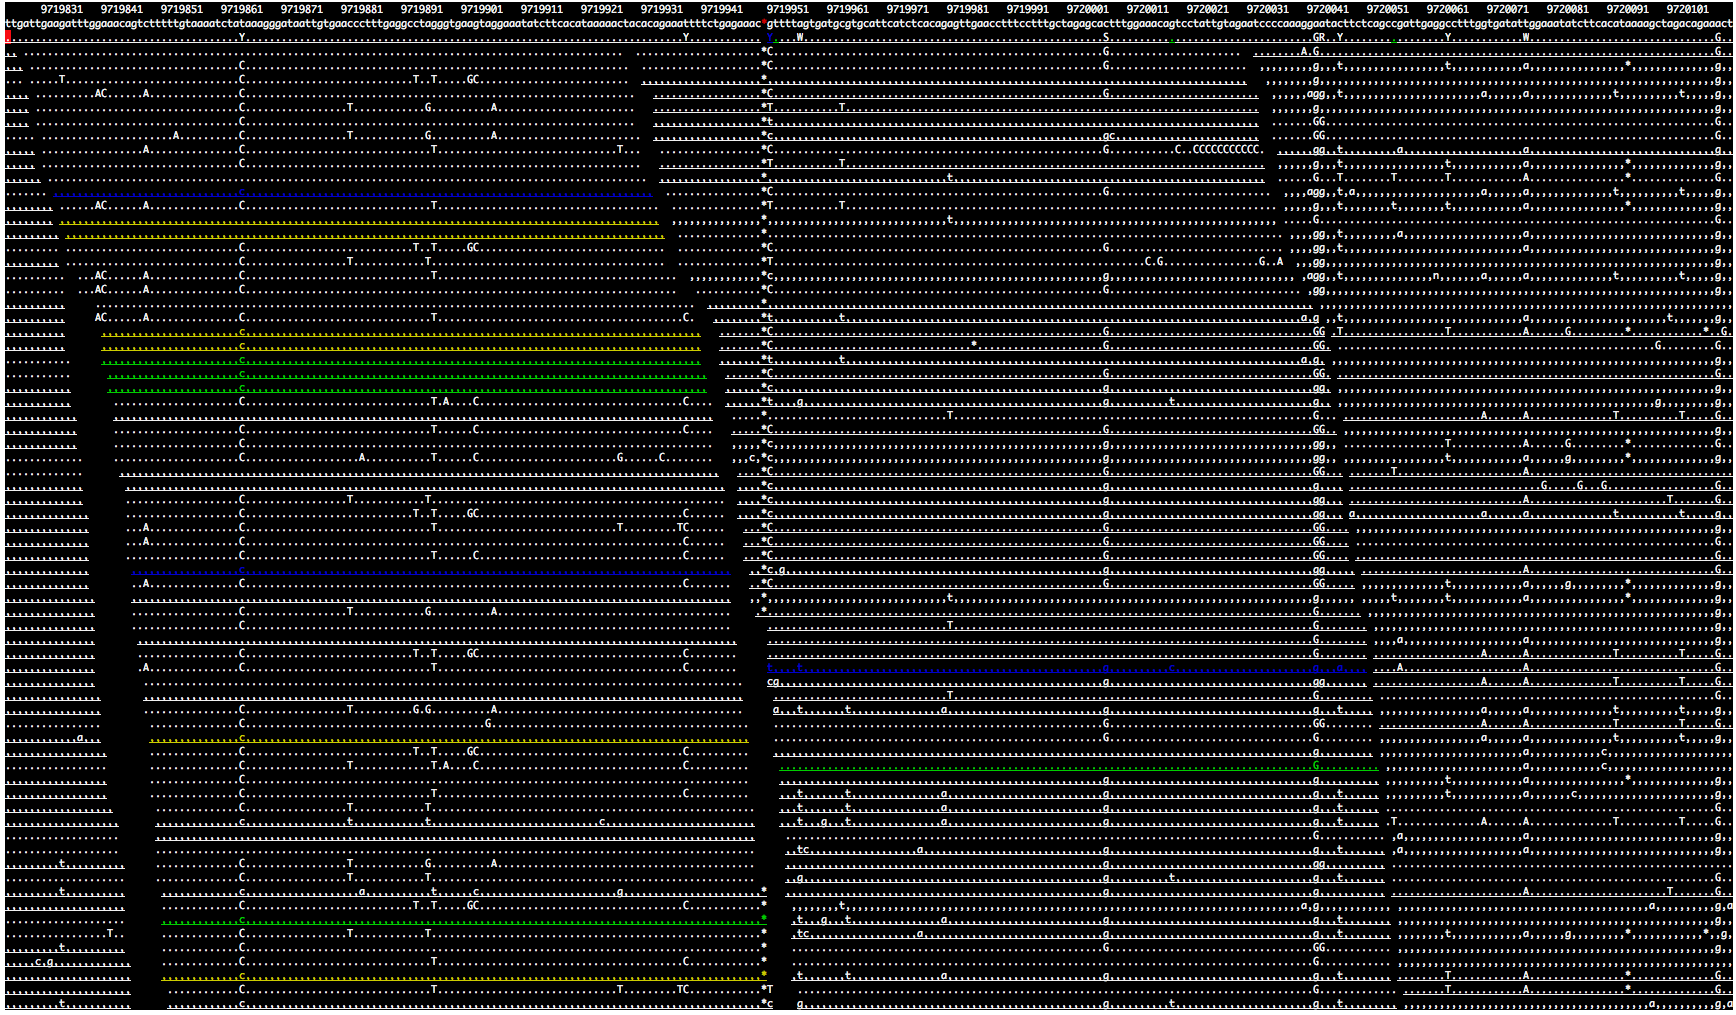
\includegraphics[height=85mm]{figs/tview_high_complexity1_veryComplex.png} 
		\caption{Different variant calling tools should be used for regions of the genome.}
	\end{figure}
\textbf{\color{berkblue}{Complexity score features:}}
\begin{table}
  \centering
  \begin{tabular*}{0.80\textwidth}{@{\extracolsep{\fill}}|l|l|p{0.5\textwidth}|}
    \hline Name & Weight & Description \\\hline
    Substitution & 3 & Number of aligned reads showing a substitution with respect to the reference.\\\hline
    Insertion & 10 & Number of aligned reads showing an insertion with respect to the reference.\\\hline
    Deletion & 10 & Number of aligned reads showing a deletion with respect to the reference.\\\hline
    Low Quality & 3 & Number of reads aligned with low map quality (a common indicator of a repetitive region).\\\hline
  \end{tabular*}
  \caption{Relative weight of features for computing complexity.}
  \label{complexity}
\end{table}
\end{block}

\vskip.75cm

\begin{block}{Results}
	\textbf{\color{berkblue}{Simulating data:}}
		\begin{itemize}
			\item Used reads simulated from the consensus sequence for Venter's genome
			\item Better approximates the true pattern of SNPs, indels, and structural variants found in a true genome; reads were aligned using BWA and SNAP %then sorted BAM files were used as input to BIGGIE
		\end{itemize}
	\textbf{\color{berkblue}{Effect of thresholds:}}
	\begin{figure}
		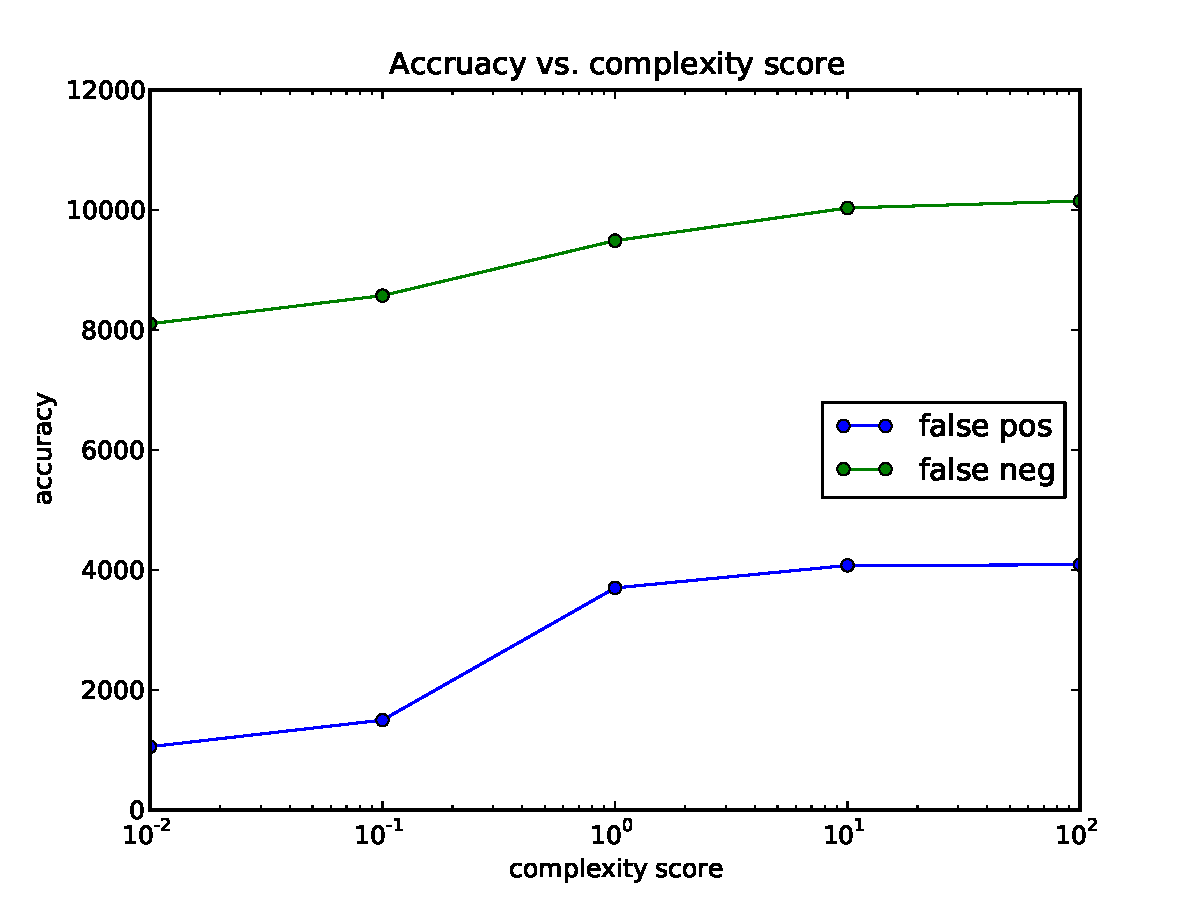
\includegraphics[height=140mm]{figs/base_accuracy_vs_thresh.pdf}
		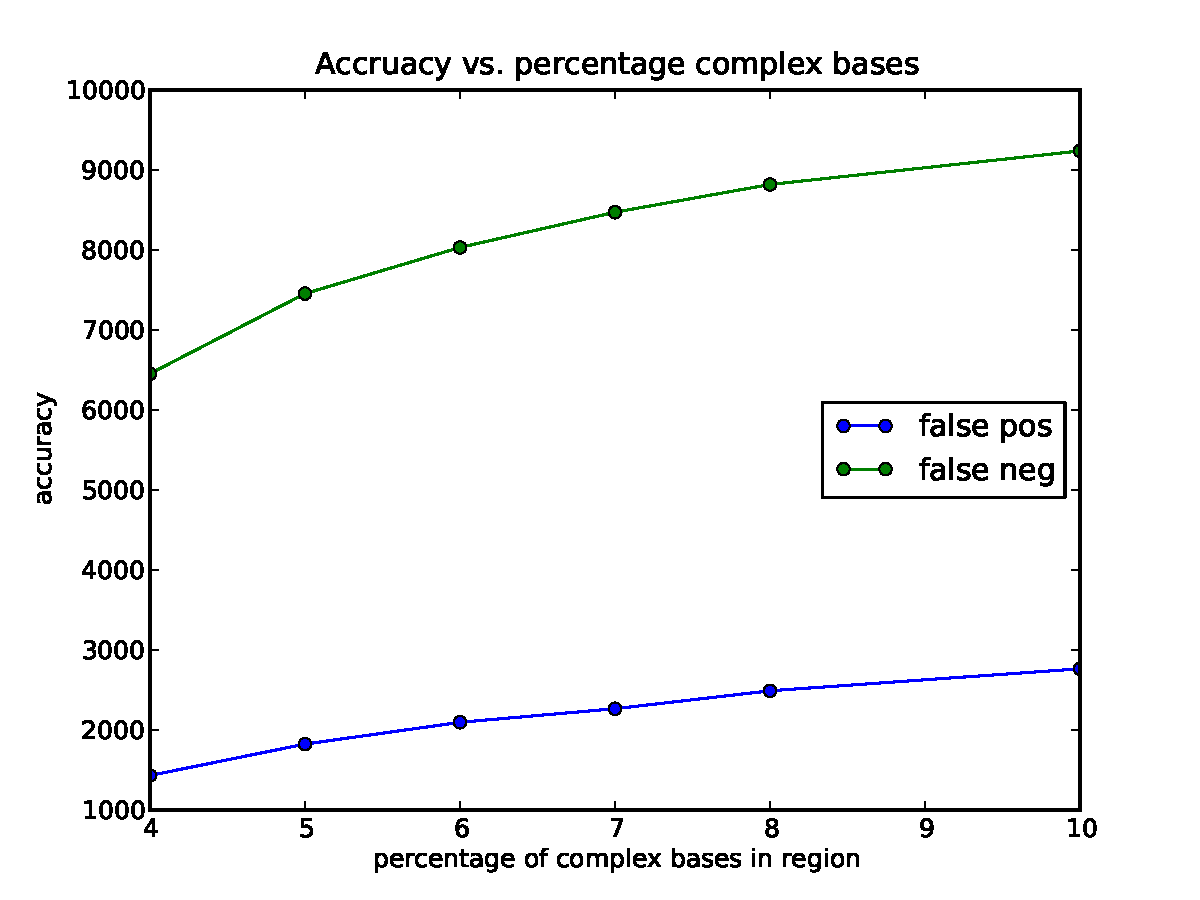
\includegraphics[height=140mm]{figs/region_accuracy_vs_thresh.pdf}
		\caption{On the left are the per-base results, measuring false negatives only on the regions we called. Both accuracy measures increase as the threshold increases, but the number of correct calls increases as well.  We see a similar pattern on the right for the region results, where the number of false positives and false negatives increase with the density of complex bases in high-complexity regions, but the number of true calls increases as well.}
	\end{figure}
\vskip-0.8cm
\end{block}

\vskip.75cm

%\begin{block}{HMM framework}
	
%\end{block}

\end{column}
\begin{column}{.48\linewidth}
      
\begin{block}{Incorporating high complexity regions}
	\begin{figure}
		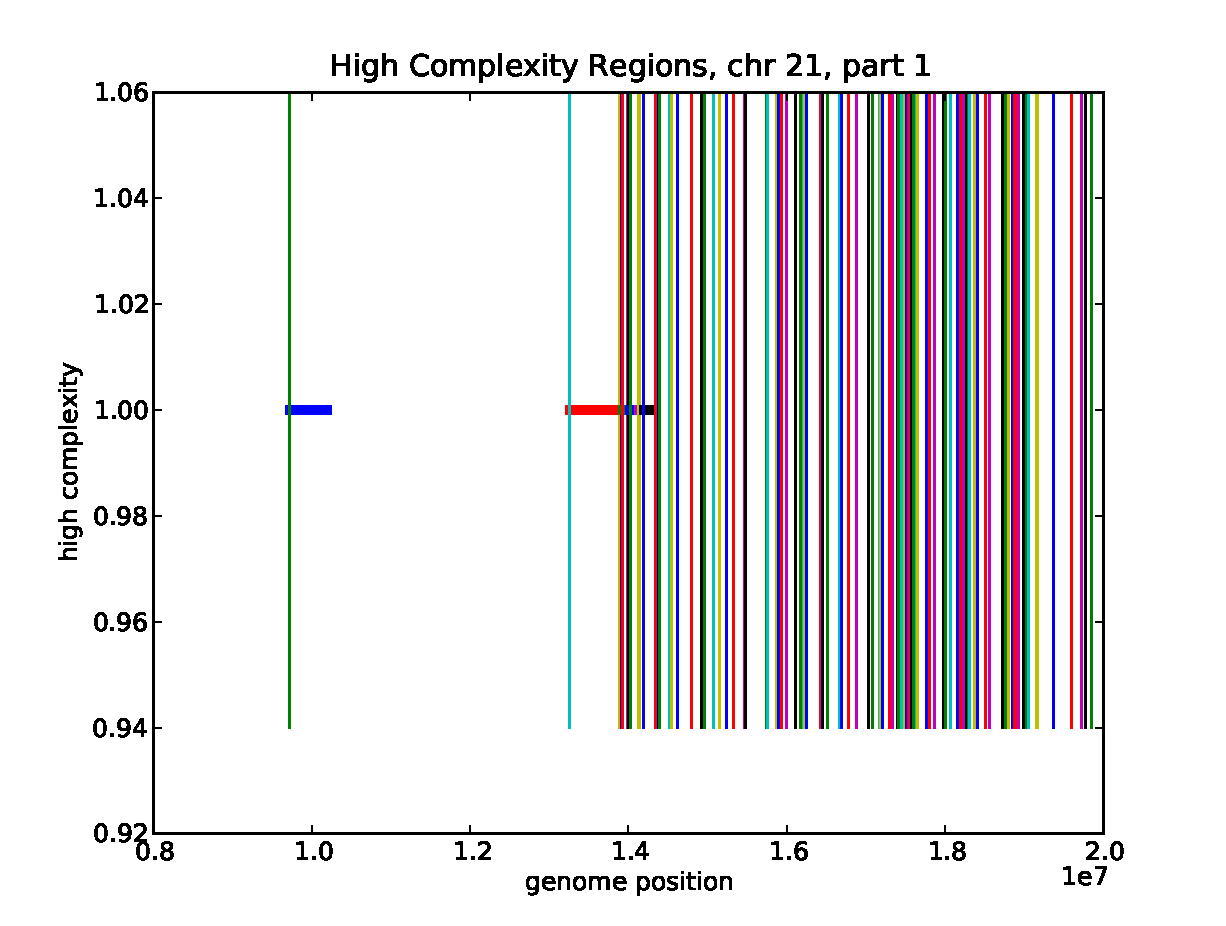
\includegraphics[height=110mm]{figs/high_complexity2_part1.pdf} 
		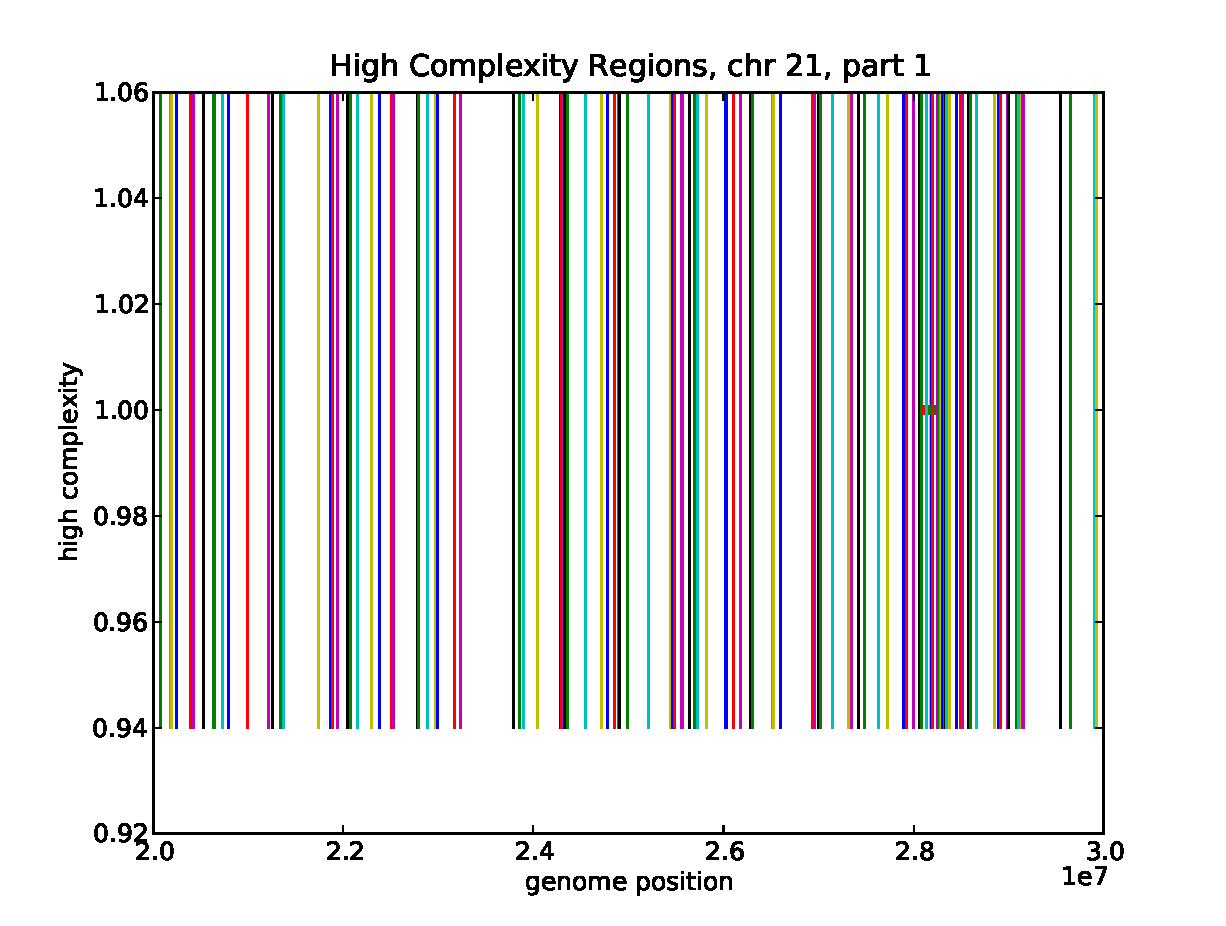
\includegraphics[height=110mm]{figs/high_complexity2_part2.pdf} 
		\caption{Regions are fairly uniformly distributed, except near the chromosome ends.}
	\end{figure}
	\vspace{2mm}
	\begin{itemize}
		\item We group bases into a high-complexity region in a greedy fashion, maintaining that the overall high-complexity base density is $>t$%, where $t$ ranges from 4\% to 10\%
		\item We filter out regions that are $<$ 500 bases long
	\end{itemize}
	\vspace{1mm}
	\begin{table}
		\begin{tabular}{|c|c|}
		\hline
		Stats, $t=5\%$ &  \\
		\hline 
 		Number of high complexity regions & 3603 \\
  		Percentage of genome is high complexity regions & 16.6\% \\
  		%Percentage of high complexity bases in high complexity regions & 15.5\% \\
		\hline
		\end{tabular}
	\end{table}
\end{block}

\vskip.75cm

\begin{block}{Results \color{berkblue}{g}}
	\vskip-0.2cm
	\begin{columns}
       	\begin{column}{.36\linewidth}
	\textbf{\color{berkblue}{Timing Results:}}
	\begin{table}
		\begin{tabular}{|c|r|}
		\hline
		Algorithm & Runtime \\
		\hline 
  		GATK & 35m 17s \\
  		mpileup & 49m 53s \\
  		BIGGIE & 4m 38s \\
		\hline
		\end{tabular}
		\caption{Timing results for GATK, mpileup, and BIGGIE. The runtime is not significantly impacted by the complexity threshold.}
	\end{table}
	\end{column}

	\begin{column}{.58\linewidth}
	\textbf{\color{berkblue}{Low vs. High Complexity:}}
	\begin{table}
		\begin{tabular}{|c|rrr|}
		\hline
		region type & false pos & false neg & correct \\
		\hline
		low-complexity & 1824 & 7455 & 38232 \\
		high-complexity & 2289 & 2788 & 13046 \\
		\hline
		\end{tabular}
		\caption{Our performance degrades in the high complexity regions, which is why a special purpose variant caller should be used.}
	\end{table}
	\end{column}

	\end{columns}

	\begin{figure}
		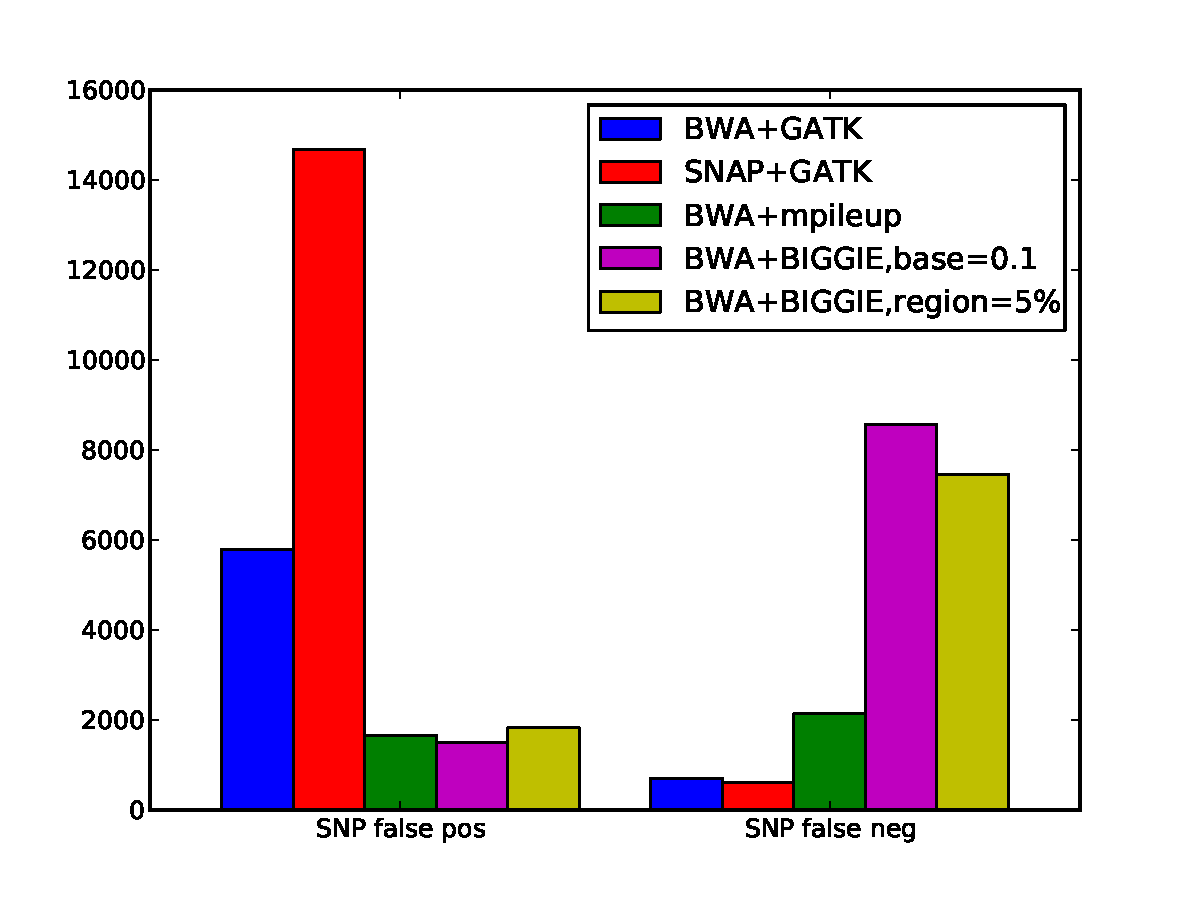
\includegraphics[width=170mm]{figs/variant_call_results_all.pdf} \hspace{5mm}
		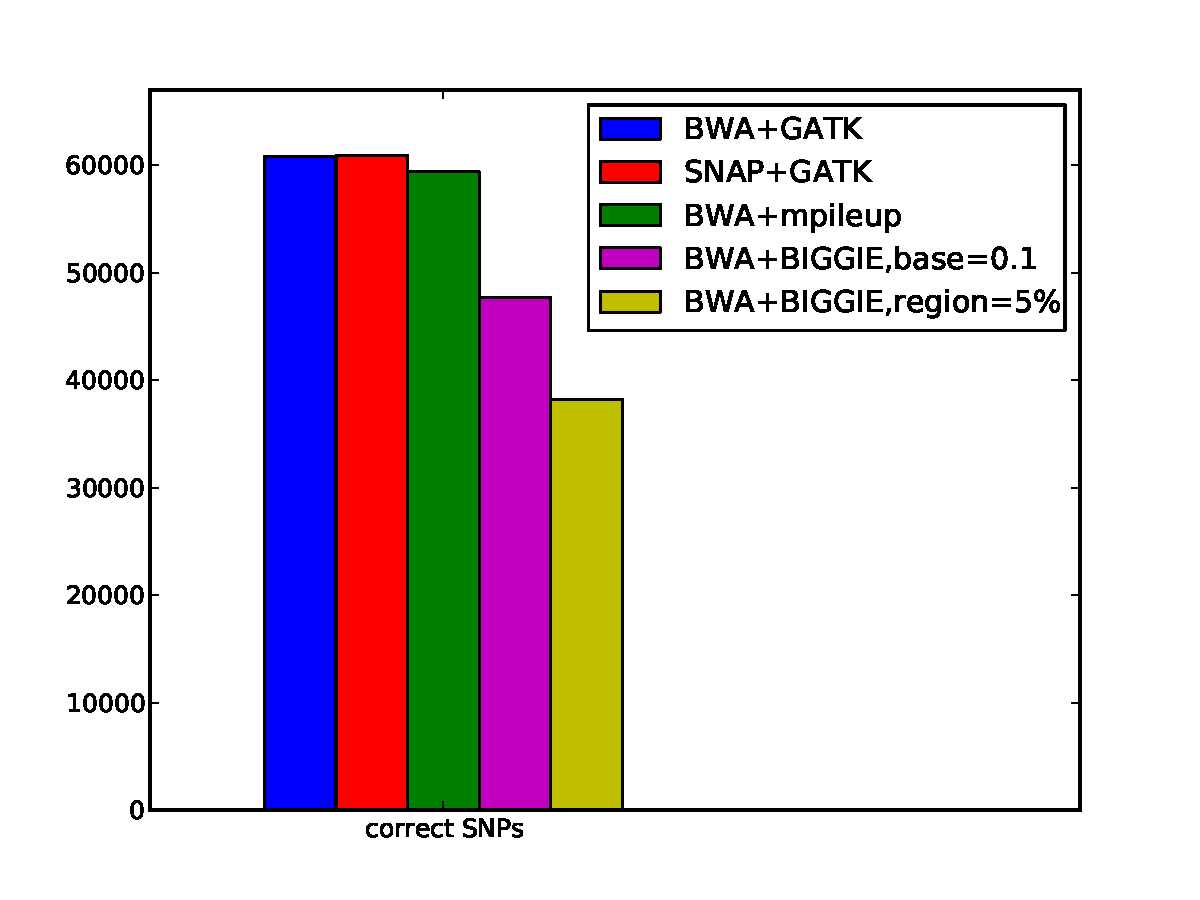
\includegraphics[width=170mm]{figs/correct_results_all.pdf}
		\caption{Accuracy comparison of BIGGIE with mpileup and GATK. False positives in BIGGIE are often associated with alignment errors or confusion with a small indel. For each algorithm, a very small percentage of correct SNP bases actually have the incorrect (unphased) genotype.} %These numbers using aligner BWA are GATK: 0.48\%, mpileup: 0.25\%, and BIGGIE: 0.35\%}
	\end{figure}
	\textbf{\color{berkblue}{Future Work:}}
	Use the high and low complexity regions to distribute the reads across machines, then call variants using appropriate algorithms.
\end{block}

\vskip.75cm

\begin{block}{References \color{berkblue}{g}}
	\vskip-0.5cm
	%\footnotesize
	\scriptsize
	[1] CASAVA. (2012) http://support.illumina.com/sequencing/sequencing\_software/casava.ilmn. \newline
	[2] DePristo M. {\em et al}, ``A framework for variation discovery and genotyping using next-generation DNA sequencing data.'' {\em Nature Genetics} (2011), 43:491-498. \newline
	[3] Li H. {\em et al} and 1000 Genome Project Data Processing Subgroup, ``The Sequence alignment/map (SAM) format and SAMtools.'' {\em Bioinformatics} (2009), 25: 2078-9. \newline
	[4] Zaharia M. {\em et al}, ``Resilient Distributed Datasets: A Fault-Tolerant Abstraction for In-Memory Cluster Computing.'' {\em NSDI} (2012).
	%\vspace{1mm}
\end{block}

\end{column}
\end{columns}

\end{frame}

\end{document}

%%%%%%%%%%%%%%%%%%%%%%%%%%%%%%%%%%%%%%%%%%%%%%%%%%%%%%%%%%%%%%%%%%%%%%%%%%%%%%%%%%%%%%%%%%%%%%%%%%%%
%%% Local Variables:
%%% mode: latex
%%% TeX-PDF-mode: t


